% This conference manuscript template is prepared for:   
% Kim Stockment, Conference Coordinator, Ray W. Herrick Laboratories, Purdue University, West Lafayette, IN, USA. 
% Latest revision = 2016-02-23 

\documentclass[10pt]{extarticle}
% Miktex users: require l3 packages
%             : optional 3 packages
\usepackage{multicol,titlesec,apacite,tabto, multirow, makecell}
%\usepackage[round]{natbib}  
\usepackage{longtable}

\usepackage[hmargin = 1in, vmargin = 1in]{geometry}

\renewcommand{\refname}{References}
    
%\usepackage[MnSymbol]{mathspec}
%\setallmainfonts{Times New Roman}
% Mathspec requires the XeTeX compiler. 


\usepackage{lineno,hyperref}
\modulolinenumbers[5]

\usepackage[T1]{fontenc}
\usepackage[utf8]{inputenc}
\usepackage{textcomp}
\usepackage{gensymb}
%%-- mwetter. \usepackage{multicol}
\usepackage{nopageno}
\usepackage{times}
\usepackage{natbib}
\usepackage{enumitem}
\usepackage[font=it]{caption}
\usepackage{doi,url}
\usepackage{hyperref}
\usepackage[usenames,dvipsnames]{xcolor}
\usepackage{listings}
\usepackage{booktabs}
\usepackage{array}
\usepackage{placeins}

%----------------------------------------------------------------%
%              Math                                              %
%----------------------------------------------------------------%

\usepackage{algorithmicx}
\usepackage{algorithm}% http://ctan.org/pkg/algorithm
\usepackage{algpseudocode}% http://ctan.org/pkg/algorithmicx
\renewcommand{\algorithmicrequire}{\textbf{INPUT:}}
\renewcommand{\algorithmicensure}{\textbf{OUTPUT:}}
\renewcommand{\algorithmicforall}{\textbf{for each}}

\usepackage{amsmath}
\usepackage{amsfonts}
\usepackage{amssymb}
\usepackage{mathtools}
\usepackage{eurosym, booktabs, units}
% \usepackage[top=2.5cm, bottom=2.5cm, left=1.5cm, right=1.5cm,
% columnsep=0.8cm]{geometry}
\usepackage{setspace}
\usepackage{fancyvrb}
\usepackage{psfrag}

%----------------------------------------------------------------%
%   FLOATS, FIGURES, TABLES, TYPOS                               %
%----------------------------------------------------------------%
\usepackage{xtab}
\usepackage{verbatim}
% \input{tikz_pck}  % TikZ graphics
% defines lengths for figure plotting
\newlength\figureheight
\newlength\figurewidth
\usepackage{tikz,pgfplots}
% \usepackage{epsfig}
\usepackage{epstopdf}
\usepackage{graphicx}
\usepackage{caption}
\usepackage{subcaption}
\usepackage{color} 
\definecolor{DarkBlue}{rgb}{0.00,0.00,0.55}
\definecolor{DarkGreen}{rgb}{0.050,0.5,0.053}

\setlength{\abovecaptionskip}{0.2cm}
\setlength{\belowcaptionskip}{0cm}
\setlength{\parindent}{0pt}

%%%% Typing commands %%%%
\newcommand{\freg}{f_{\Theta}}
\newcommand{\mbbox}{\ensuremath{\rule{0pt}{0pt}\hfill
    \text{{\scriptsize $\blacksquare$}}}}
\newcommand{\mwbox}{\ensuremath{\rule{0pt}{0pt}\hfill
    \text{{\scriptsize $\square$}}}} 
\DeclarePairedDelimiter{\abs}{\lvert}{\rvert}
% MPC formulation
\newcommand{\lrp}[1]{\ensuremath{\left( #1 \right)}}
\newcommand{\QQ}[1]{Q_{\text{#1}}}
\newcommand{\phm}{\phantom{-}}

\newtheorem{remark}{Remark}

\usepackage{changepage}  % allows to use adjustwidth

\usepackage{titlesec} 
%\titleformat{command}[shape]{format}{label}{sep}{before}[after]
\titleformat{\section}[hang]{\fontsize{12pt}{1em}\selectfont \bfseries}{\thesection. }{0pt}{\centering \MakeUppercase}
\titleformat{\subsection}[hang]{\fontsize{11pt}{1em}\selectfont \bfseries}{\thesubsection}{5pt}{}
\titleformat{\subsubsection}[runin]{}{\thesubsubsection}{5pt}{} 
%\titlespacing{command}{left}{beforesep}{aftersep}[right]
\titlespacing{\section}{0pt}{10pt}{10pt}
\titlespacing{\subsection}{0pt}{10pt}{0pt}
\titlespacing{\subsubsection}{0pt}{10pt}{0pt}	
%\setlength{\bibsep}{3pt}
%\pagenumbering{\gobble}
%\setlength{\hyphenpenalty}{1000}
%\setlength{\exhyphenpenalty}{1000}

\usepackage{fancyhdr}
\pagestyle{fancy}
\fancyhead[R]{\fontsize{12pt}{1em}\selectfont {{\textbf{Page \thepage}}}}
\fancyhead[L]{}
\fancyfoot[C]{IBPSA Project 1, September 2018}
\renewcommand{\headrulewidth}{0pt} % Turn off the bar

\newcommand\thefontsize[1]{{#1 The current font size is: \f@size pt\par}}


\begin{document}
	
\begin{center}
\vspace{0.2in}
\noindent{\fontsize{14pt}{1em}\selectfont \textbf{MPC formulation description template -- An example}}\\[14pt]

{\fontsize{11pt}{1.2em}\selectfont
 J\'an Drgo\v na\textsuperscript{1}
\\[11pt]

KU Leuven\\
Department of Mechanical Engineering - TME Division\\
Thermal Systems Simulation  (The SySi) research group  \\[11pt]

jan.drgona@kuleuven.be\textsuperscript{1}\\
}
\end{center}

\vspace{0.5cm}


\section*{Abstract}

This document presents an example of the MPC formulation, using IBPSA Project 1 template.
Twelve-zone office building is used for demonstation of the methodology.
General description of the building is follosed by definition of key performance indicators (KPIs) and physical constraints.
Equivalence of MPC formulations using physical notation and control engineering notation is demonstrated using translation template.

\section{Building Description}\label{sec:building}
Building envelope and HVAC.
% 
\begin{figure}[htbp]
\centering
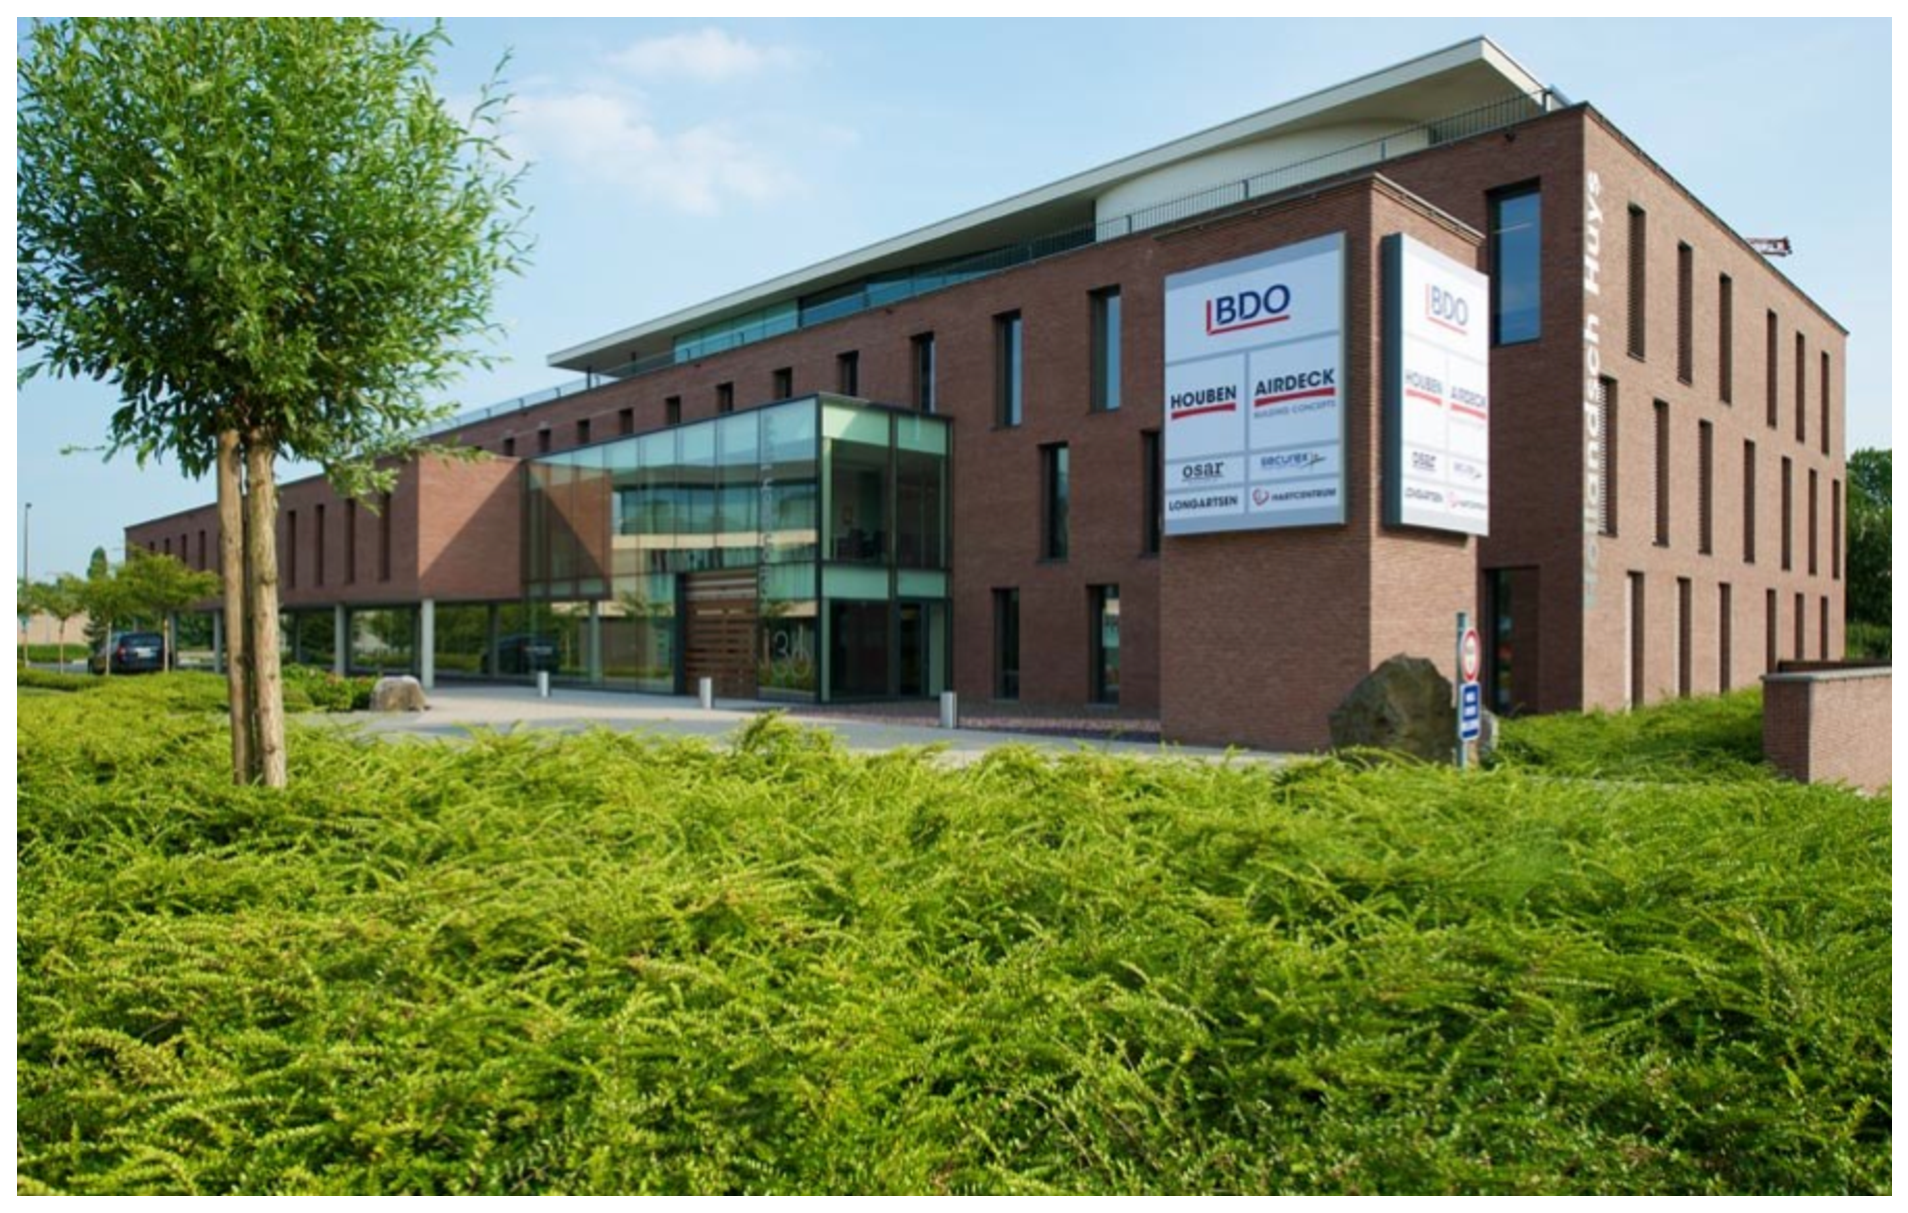
\includegraphics[width=0.80 \textwidth]{fig/HH_building.eps}
\caption{Hollandsch Huys office building.
}
\label{fig:approxMPC:TDNN}
\end{figure}
%
\begin{figure}[htbp]
\centering
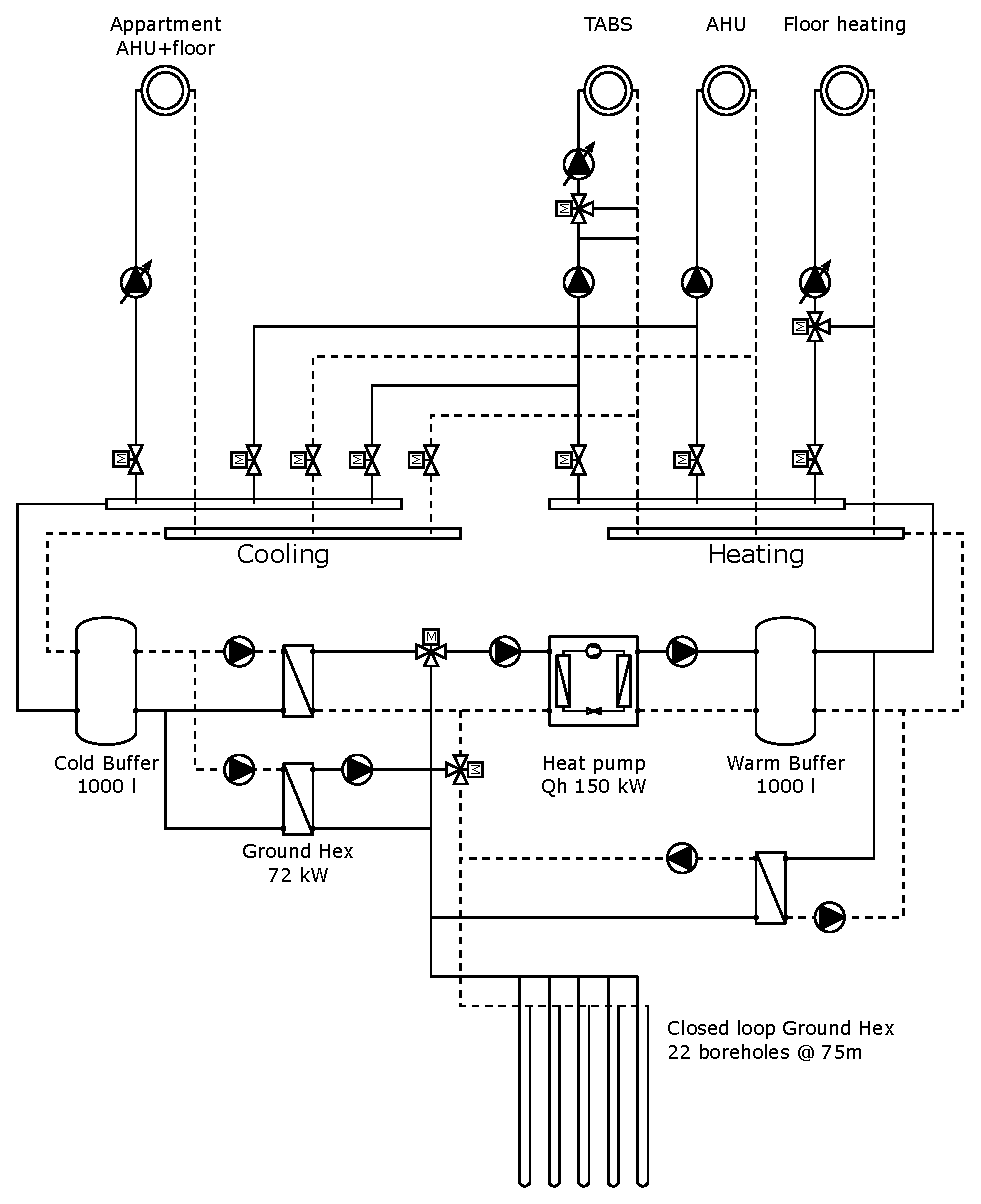
\includegraphics[width=0.80 \textwidth]{fig/HH_HVAC.eps}
\caption{Hollandsch Huys heating system scheme.
}
\label{fig:approxMPC:TDNN}
\end{figure}


\section{Variables and Parameters}\label{sec:variables}
% 
Variables and parameters used in Hollandsch Huys.
% 
\begin{table}[htbp!]
	% Suppressing floating placement of tables/figures in LaTeX is generally deprecated. 
	\centering
	\caption{MPC variables notation and translation between physical and abstract domain. }
	\label{tab:mpc_form:translation}
% 	\begin{adjustwidth}{-1cm}{}
	\begin{tabular}{l|c|l|cccc}
		\toprule
		\multicolumn{3}{l}{\textbf{Physical domain}} &  \multicolumn{4}{r}{\textbf{Abstract domain}} \\
		\toprule
		\textbf{Variables} & \textbf{Symbol} & \textbf{Description} & \textbf{$x$} & \textbf{$y$} & \textbf{$u$} & \textbf{$d$}  \\ 
		\midrule
		\multirow{8}{*}{\textbf{Temperatures [$^\circ C$]}} & $T$ & Envelope temperatures (wall, concrete, glazing...) & $\bullet$ & -  & - & - \\ 
		& $T_{\text{z}}$ & Zone operative temperatures  & - & $\bullet$ & -  & - \\
		& $T^{\text{AHU}}_{\text{sup}}$ & Air supply temperatures AHU &  - & - & - & $\bullet$ \\
		& $T^{\text{HP}}_{\text{sup}}$ & Water supply temperatures heat pump&  - & - & - & $\bullet$ \\
		& $T^{\text{TABS}}_{\text{sup}}$ & Water supply temperatures TABS&  - & - & $\bullet$ & -  \\
% 		& $T^{\text{FH}}_{\text{sup}}$ & Water supply temperatures floor heating&  - & - & $\bullet$ & -  \\
		& $T^{\text{TABS}}_{\text{ret}}$ & Water return temperature TABS &  - & - & - & $\bullet$ \\
% 		& $T^{\text{FH}}_{\text{ret}}$ & Water return temperature floor heating &  - & - & - & $\bullet$  \\
		& $T_\text{e}$ & Ambient temperature &  - & - & - & $\bullet$ \\
		\midrule
		\multirow{3}{*}{\textbf{Thermal power $[W]$}} 
		& $\dot{Q}_{\text{HVAC}}$ & Thermal power of  HVAC components  & - & - &  $\bullet$ &- \\
		& $\dot{Q}_{\text{rad}}$ & Solar radiation & - & - & - & $\bullet$  \\
		& $\dot{Q}_{\text{occ}}$ & Occupancy internal gains & - & - & - & $\bullet$  \\
\midrule
		\multirow{2}{*}{\textbf{Mass flows $[kg/s]$}} &
		$\dot{m}_{\text{wat}}$ & Water mass flow in & - & - & - & $\bullet$ \\
		&  & TABS and floor heating  & &  &  \\
		\midrule
		\multirow{3}{*}{\textbf{\shortstack[l]{Component signals }}} 
% 		& $x_{\text{HVAC}}$ & ON/OFF/Modulated signal of HVAC components $[\{0,1\},\%]$ & - & - & $\bullet$ & - \\
		& $x_{\text{TABS}}$ & ON/OFF signal of TABS pump $[\{0,1\}]$ & - & - & $\bullet$ & - \\
% 		& $x_{\text{FH}}$ & ON/OFF signal of floor heating pump $[\{0,1\}]$ & - & - & $\bullet$ & - \\
		& $x_{\text{val}}$ & Valve positions TABS $[\%]$ & - & - & $\bullet$ & - \\
		& $x_{\text{heat}}$ & ON/OFF heating mode $[\{0,1\}]$ & - & - & $\bullet$ & - \\
		& $x_{\text{cool}}$ & ON/OFF cooling mode $[\{0,1\}]$ & - & - & $\bullet$ & - \\
		\bottomrule 
	\end{tabular}
% 	 \end{adjustwidth}
\end{table} 
% 
\renewcommand{\arraystretch}{2}
\begin{table}[htbp]
	% Suppressing floating placement of tables/figures in LaTeX is generally deprecated. 
	\centering
	\caption{MPC formulation parameters - modifiers and auxiliary variables.}
	\label{tab:mpc_form:parameters:modifiers}
	\begin{tabular}{l|c|l|c}
		\toprule
		\textbf{Energy efficiencies}  & \textbf{Symbol} &  \textbf{Description} & \textbf{Associated variables} \\
		\midrule
		\makecell[l]{Coefficient of \\ performance} & $COP$ &  \makecell[l]{Coefficient of performance \\ of heat pump} & $\dot{Q}_{\text{HVAC}}$ \\
		\midrule
		\textbf{Other energy factors}  & \textbf{Symbol} &  \textbf{Description} & \textbf{Associated variables} \\
		\midrule
		Price factor & $p$ &  \makecell[l]{Conversion factor from energy \\ to monetary cost} & $\dot{Q}_{\text{HVAC}}$ \\
			\midrule
		\textbf{Heat flow parameters}  & \textbf{Symbol} &  \textbf{Description} & \textbf{Associated variables} \\
		\midrule
		Specific heat capacity & $c_p$ & \makecell[l]{Specific heat capacity of water} & $T_{sup}, T_{ret}, \dot{m}_{\text{wat}}, \dot{Q}^i_{\text{HVAC}}$ \\
		\midrule
		\textbf{Auxiliary parameters}  & \textbf{Symbol} &  \textbf{Description} & \textbf{Associated variables} \\
		\midrule
        \makecell[l]{Slack variable} & $s$ &  \makecell[l]{Used to soften the constraints, usually \\ for the given comfort requirement} 
		&  all \\
		\makecell[l]{Weighting factor} & $Q_{\star}$ &  \makecell[l]{Weighting for the particular term \\ in the objective function} & all \\
		\makecell[l]{Sampling time} & $T_s$ &  \makecell[l]{Time-step used in the \\ optimization problem} & all  \\
		\makecell[l]{Dimensionality quantifier} & $n_{\star}$ &  \makecell[l]{Cardinality of the vector elements} & all \\
		\bottomrule 
	\end{tabular}
\end{table}
% 
\renewcommand{\arraystretch}{2}
\begin{table}[htbp]
	% Suppressing floating placement of tables/figures in LaTeX is generally deprecated. 
	\centering
	\caption{MPC formulation parameters - bounds and references $r$.}
	\label{tab:mpc_form:parameters:bounds}
% 		\begin{adjustwidth}{-1.5cm}{}
	\begin{tabular}{l|c|l|c}
		\toprule
		\textbf{Comfort bounds $r$}  & \textbf{Symbol} &  \textbf{Description} & \textbf{Associated variables} \\
		\midrule
		Temperature & $\underline{T}_{\text{z}},\overline{T}_{\text{z}}$ & \makecell[l]{Zone operative temperature  \\ comfort bounds } & $T_{\text{z}}$ \\
		\bottomrule 
		\textbf{Component limitations}  & \textbf{Symbol} &  \textbf{Description} & \textbf{Associated variables} \\
		\midrule
		Thermal power limit & $\underline{\dot{Q}}^i_{\text{HVAC}},\overline{\dot{Q}}^i_{\text{HVAC}}$ & \makecell[l]{Min/max thermal power of \\ the $i$-th HVAC component} & $Q^i_{\text{HVAC}}$ \\
% 		\makecell[l]{Rate of change of\\ thermal power rate}  & $\underline{\Delta \dot{Q}^i_{\text{HVAC}}},\overline{\Delta \dot{Q}^i_{\text{HVAC}}}$ & \makecell[l]{Min/max rate of change of  thermal  \\ power  of the  $i$-th HVAC component} & $Q^i_{\text{HVAC}}$ \\
		Valve position limits & $\underline{ x}^i_{\text{val}},\overline{ x}^i_{\text{val}}$ & \makecell[l]{Min/max position of \\  the  $i$-th valve} & $x^i_{\text{val}}$ \\
% 		\makecell[l]{Rate of change of\\ valve position}  & $\underline{\Delta x^i_{\text{val}}},\overline{\Delta x^i_{\text{val}}}$ & \makecell[l]{Min/max change of \\ position of the  $i$-th valve} & $x^i_{\text{val}}$ \\
		\bottomrule 
	\end{tabular}
% 	\end{adjustwidth}
\end{table}



% \section{KPIs and Constraints}\label{sec:variables}


\section{MPC Formulation: Physical Notation}\label{sec:physical_notation}


% TODO MPC notation with physical vartiables


The MPC minimizing  the energy consumption and  thermal discomfort 
for Hollandsch Huys building is given as the following quadratic optimization problem using physical notation:
\begin{subequations}
\label{eq:mpc_general}
\begin{align}
 \min_{\dot{Q}_{\text{HVAC},0}, \ldots, \dot{Q}_{\text{HVAC},{N_{\text{c}}-1}},
 s^{T_{\text{z}}}_0, \ldots, s^{T_{\text{z}}}_{N-1}} & \sum_{k=0}^{N-1}  
 || s^{T_{\text{z}}}_k ||_{Q_\text{s}}^2 +  \sum_{k=0}^{N_{\text{c}}-1} COP_k p_k ||\dot{Q}_{\text{HVAC},k} ||_{Q_\text{u}}^2  &
 \label{eq:mpc_general:cost}\\
  \text{s.t.} \ & T_{k+1} = A T_k+ B \dot{Q}_{\text{HVAC},k} +E [\dot{Q}_{\text{rad},k}, \dot{Q}_{\text{occ},k}, T_{\text{e},k}]^T, & k \in \mathbb{N}_{0}^{N-1} \label{eq:mpc_general:x} \\
  & T_{\text{z},k} = C T_k + D \dot{Q}_{\text{HVAC},k}, & k \in \mathbb{N}_{0}^{N-1} \label{eq:mpc_general:y} \\
  & \underline{T}_{\text{z},k} - s^{T_{\text{z}}}_k \le T_{\text{z},k} \le \overline{T}_{\text{z},k} + s^{T_{\text{z}}}_k, & k \in \mathbb{N}_{0}^{N-1} \label{eq:mpc_general:zone} \\
   & \mathbf{0} \le s^{T_{\text{z}}}_k  ,  & k \in \mathbb{N}_{0}^{N-1} \label{eq:mpc_general:lb_sk}\\
    & \dot{Q}_{\text{HVAC},k} =  \begin{cases}
    \dot{Q}_{\text{HVAC},k} & \text{if } k \leq N_{\text{c}}\\
   \dot{Q}_{\text{HVAC},N_{\text{c}}}     & \text{otherwise}   \end{cases}, & k \in \mathbb{N}_{0}^{N-1} \label{eq:mpc_general:move_block} \\
  &  \underline{\dot{Q}}_{\text{HVAC},k} \le \dot{Q}_{\text{HVAC},k} \le \overline{\dot{Q}}_{\text{HVAC},k},  & k \in \mathbb{N}_{0}^{N-1} \label{eq:mpc_general:ub}\\
   & \dot{Q}_{\text{rad},k} =  \dot{Q}_{\text{rad}}(t+ k T_s), & k \in \mathbb{N}_{0}^{N-1} \label{eq:mpc_general:d0} \\
   & \dot{Q}_{\text{occ},k} = \dot{Q}_{\text{occ}}(t+ k T_s), & k \in \mathbb{N}_{0}^{N-1} \label{eq:mpc_general:d0} \\
   & T_{\text{e},k} = T_{\text{e}}(t+ k T_s), & k \in \mathbb{N}_{0}^{N-1} \label{eq:mpc_general:d0} \\
  & \underline{T}_{\text{z},k} =  \underline{T}_{\text{z}}(t+ k T_s), & k \in \mathbb{N}_{0}^{N-1} \label{eq:mpc_general:r_low} \\
    & \overline{T}_{\text{z},k} =  \overline{T}_{\text{z}}(t+ k T_s), & k \in \mathbb{N}_{0}^{N-1} \label{eq:mpc_general:r_up} \\
  & T_0 = \hat{T}(t) \label{eq:mpc_general:x0}
%   & \forall k \in \{0, \ldots, N-1\}. \label{eq:mpc_general:k}
\end{align}
\end{subequations}
where $\mathbb{N}_a^b = \{a, a+1, \ldots, b \}$ is a set of integers,
$T_k$, $u_k$, $y_k$ and $d_k$ represent the values of the zone temperatures, 
inputs, outputs and disturbances, respectively, 
predicted at the $k$-th step of the prediction horizon $N$.
The predictions are obtained from the LTI prediction
model given by equations~\eqref{eq:mpc_general:x} and~\eqref{eq:mpc_general:y}.
The $\underline{T}_{\text{z},k}$ and $\overline{T}_{\text{z},k}$ parameters represent the comfort band 
given by the constraints~\eqref{eq:mpc_general:zone},
where the variables $s^{T_{\text{z}}}_k$ are used as the slack variables of a comfort band violation.
The min/max constraints for the control input amplitude are given by~\eqref{eq:mpc_general:ub}.
For particular initial conditions~\eqref{eq:mpc_general:x0} and~\eqref{eq:mpc_general:d0}, 
 the optimization computes the sequence $\dot{Q}_{\text{HVAC},k}^*, \ldots, \dot{Q}_{\text{HVAC},N_{\text{c}-1}}^*$ of control inputs that
are optimal with respect to the quadratic objective function~\eqref{eq:mpc_general:cost}
and the constraints.
The term $\|a\|_Q^2$ in the objective function represents the weighted squared $2$-norm, i.e., $a^T Q a$,
with the weighting matrices $Q_\text{s}$ and $Q_\text{u}$ given as positive 
definite diagonal matrices.
The first term of the quadratic cost function minimizes the square of the comfort violation,
while the second term minimizes the square of the used energy.


Due to the linearization of the model, the decision variables represent heat flows delivered to the building $\dot{Q}_{\text{HVAC},k}$. However, in practical setup, we are not able to directly control the heat flows. Instead, we need to optimally map the heat computed by MPC to the physical control variables. In particular, we can control $20$ two way valves of individual circuits of thermally activated building structures (TABS) denoted by variable $x_{\text{val}}$, and supply temperature for TABS denoted by $T^{\text{TABS}}_{\text{sup}}$. We compute these values by solving nonlinear optimization problem (NLP) with heat transfer equation, minimizing the difference between supply and return temperatures for TABS, opening  of the valves, and  penalizing the deviation from satisfaction of the heat transfer equation via slack variables $s$. Specific heat capacity of the water $c_p$ and nominal mass flow rates $\dot{m}_{\text{wat}}$ obtained from the technical sheets of the building are used as constant parameters. The measurements of return temperatures from TABS circuits $T^{\text{TABS}}_{\text{ret}}$, supply temperature from heat pump $T^{\text{HP}}_{\text{sup}}$ the the  and computed optimal heat flows $\dot{Q}_{\text{HVAC},k}$ are used as varying parameters for corresponding NLP:
\begin{subequations}
\label{eq:NLP_postprocess}
\begin{align}
 \min_{x_{\text{val},k}, T_{\text{sup},k}^{\text{TABS}}} &  \sum_{i=1}^{n_{\text{TABS}}} \lrp{(T_{\text{sup},k}^{\text{TABS}} - T_{\text{ret},k}^{\text{TABS},i}) + x_{\text{val},k}^i } +  || s_{k}^{\text{TABS}} ||_{Q^{\text{TABS}}_{\text{s}}}^2 &
 \label{eq:NLP_postprocess:cost}\\
  \text{s.t.} \ &  \dot{Q}_{\text{HVAC},k} + s_{k}^{\text{TABS}} = x_{\text{val},k} \ \dot{m}_{\text{wat}} \ c_p \ (T_{\text{sup},k}^{\text{TABS}} -  T_{\text{ret},k}^{\text{TABS},i}), &  \label{eq:NLP_postprocess:heat_equation} \\
   &  T_{\text{ret},k}^{\text{TABS}} \le T_{\text{sup},k}^{\text{TABS}} \le T_{\text{sup},k}^{\text{HP}}, \label{eq:NLP_postprocess:tsup_minmax}\\
    & \underline{x}^i_{\text{val}} \le x_{\text{val},k} \le \overline{x}^i_{\text{val}}.   \label{eq:NLP_postprocess:valve_minmax}
\end{align}
\end{subequations}

% \begin{subequations}
% \label{eq:NLP_postprocess}
% \begin{align}
%  \min_{x_{\text{val}}, T_{\text{sup},k}^{\text{TABS}}} & \sum_{k=0}^{N-1} \lrp{ \sum_{i=1}^{n_{\text{TABS}}} \lrp{(T_{\text{sup},k}^{\text{TABS}} - T_{\text{ret},k}^{\text{TABS},i}) + x_{\text{val},k}^i } +  || s_{k}^{\text{TABS}} ||_{Q^{\text{TABS}}_{\text{s}}}^2  }&
%  \label{eq:NLP_postprocess:cost}\\
%   \text{s.t.} \ &  \dot{Q}_{\text{HVAC},k} + s_{k}^{\text{TABS}} = x_{\text{val},k} \ \dot{m}_{\text{wat}} \ c_p \ (T_{\text{sup},k}^{\text{TABS}} -  T_{\text{ret},k}^{\text{TABS},i}), &  \label{eq:NLP_postprocess:heat_equation} \\
%    &  T_{\text{ret},k}^{\text{TABS}} \le T_{\text{sup},k}^{\text{TABS}} \le T_{\text{sup},k}^{\text{HP}}, \label{eq:NLP_postprocess:tsup_minmax}\\
%     & 0 \le x_{\text{val},k} \le 1.   \label{eq:NLP_postprocess:valve_minmax}
% \end{align}
% \end{subequations}

\section{MPC Formulation: Control Engineering Notation}\label{sec:control_notation}


The MPC minimizing  the energy consumption and  thermal discomfort 
for Hollandsch Huys building is given as the following quadratic optimization problem using control engineering notation:
\begin{subequations}
\label{eq:mpc_general}
\begin{align}
 \min_{u_0, \ldots, u_{N_{\text{c}}-1}, s_0, \ldots, s_{N-1}} & \sum_{k=0}^{N-1}  
 || s_k ||_{Q_\text{s}}^2 +  \sum_{k=0}^{N_{\text{c}}-1} COP_k p_k ||u_k ||_{Q_\text{u}}^2  &
 \label{eq:mpc_general:cost}\\
  \text{s.t.} \ & x_{k+1} = A x_k+ B u_k +E d_k, & k \in \mathbb{N}_{0}^{N-1} \label{eq:mpc_general:x} \\
  & y_{k} = C x_k + D u_k, & k \in \mathbb{N}_{0}^{N-1} \label{eq:mpc_general:y} \\
  & \underline{y}_k - s_k \le y_k \le \overline{y}_k + s_k, & k \in \mathbb{N}_{0}^{N-1} \label{eq:mpc_general:zone} \\
   & \mathbf{0} \le s_k  ,  & k \in \mathbb{N}_{0}^{N-1} \label{eq:mpc_general:lb_sk}\\
    & u_k =  \begin{cases}
    u_k & \text{if } k \leq N_{\text{c}}\\
   u_{N_{\text{c}}}     & \text{otherwise}   \end{cases}, & k \in \mathbb{N}_{0}^{N-1} \label{eq:mpc_general:move_block} \\
  & \underline{u} \le u_k \le \overline{u},  & k \in \mathbb{N}_{0}^{N-1} \label{eq:mpc_general:ub}\\
   & d_k = d(t+ k T_s), & k \in \mathbb{N}_{0}^{N-1} \label{eq:mpc_general:d0} \\
  & \underline{y}_k =  \underline{y}(t+ k T_s), & k \in \mathbb{N}_{0}^{N-1} \label{eq:mpc_general:r_low} \\
    & \overline{y}_k =  \overline{y}(t+ k T_s), & k \in \mathbb{N}_{0}^{N-1} \label{eq:mpc_general:r_up} \\
  & x_0 = \hat{x}(t) \label{eq:mpc_general:x0}
%   & \forall k \in \{0, \ldots, N-1\}. \label{eq:mpc_general:k}
\end{align}
\end{subequations}
where $\mathbb{N}_a^b = \{a, a+1, \ldots, b \}$ is a set of integers,
$x_k$, $u_k$, $y_k$ and $d_k$ represent the values of the states, 
inputs, outputs and disturbances, respectively, 
predicted at the $k$-th step of the prediction horizon $N$.
The predictions are obtained from the LTI prediction
model given by equations~\eqref{eq:mpc_general:x} and~\eqref{eq:mpc_general:y}.
The $lb_k$ and $ub_k$ parameters represent the comfort band 
given by the constraints~\eqref{eq:mpc_general:zone},
where the variables $s_k$ are used as the slack variables of a comfort band violation.
The min/max constraints for the control input amplitude are given by~\eqref{eq:mpc_general:ub}.
For particular initial conditions~\eqref{eq:mpc_general:x0} and~\eqref{eq:mpc_general:d0}, 
 the optimization computes the sequence $u_0^*, \ldots, u_{N-1}^*$ of control inputs that
are optimal with respect to the quadratic objective function~\eqref{eq:mpc_general:cost}
and the constraints.
The term $\|a\|_Q^2$ in the objective function represents the weighted squared $2$-norm, i.e., $a^T Q a$,
with the weighting matrices $Q_\text{s}$ and $Q_\text{u}$ given as positive 
definite diagonal matrices.
The first term of the quadratic cost function minimizes the square of the comfort violation,
while the second term minimizes the square of the used energy.
% 

% TODO
Control engineering notation of NLP post-processing follows:
\begin{subequations}
\label{eq:NLP_postprocess}
\begin{align}
 \min_{x_{\text{val},k}, T_{\text{sup},k}^{\text{TABS}}} & \sum_{i=1}^{n_{\text{TABS}}} \lrp{(T_{\text{sup},k}^{\text{TABS}} - T_{\text{ret},k}^{\text{TABS},i}) + x_{\text{val},k}^i } + || s_{k}^{\text{TABS}} ||_{Q^{\text{TABS}}_{\text{s}}}^2  &
 \label{eq:NLP_postprocess:cost}\\
  \text{s.t.} \ & u_k + s_{k}^{\text{TABS}} = x_{\text{val},k} \ \dot{m}_{\text{wat}} \ c_p \ (T_{\text{sup},k}^{\text{TABS}} -  T_{\text{ret},k}^{\text{TABS},i}), &  \label{eq:NLP_postprocess:heat_equation} \\
   &  T_{\text{ret},k}^{\text{TABS}} \le T_{\text{sup},k}^{\text{TABS}} \le T_{\text{sup},k}^{\text{HP}}, \label{eq:NLP_postprocess:tsup_minmax}\\
     & \underline{x}^i_{\text{val}} \le x_{\text{val},k} \le \overline{ x}^i_{\text{val}}.   \label{eq:NLP_postprocess:valve_minmax}
\end{align}
\end{subequations}


% TODO add post processing NLP
% TODO comments with links to physical notation


\section*{Acknowledgements}

This work emerged from the IBPSA Project 1, an international project conducted under the umbrella of the International Building Performance Simulation Association (IBPSA). Project 1 will develop and demonstrate a BIM/GIS and Modelica Framework for building and community energy system design and operation.

The authors acknowledge the financial support by the European Union through  the EU-H2020-GEOT\euro CH 
project ‘Geothermal Technology for \euro conomic Cooling and Heating’.

\end{document}
